\section{Analysis}

\subsection{Comparison Methods}

Our main means of analysis was to compare algorithm performance over different numbers of sensors and different numbers of sectors. The number of sectors was the same for each sensor for each test, but could vary from test to test.

After building and testing the graphical environment, we set it up to execute batches of tests independant of the graphical interface. This allowed us to collect a lot of data quickly.

Specifically the batch runs would be for a particular number of sensors passed in as a command line argument. A second argument t is used for the number of tests to be run. The tests are run t times for each algorithm running over the k (number of sectors) values from 3 to 12. Log files are generated as well as statistical files. The statistical files are performance numbers formatted for graph generation. 
This data is then run through an averaging algorithm which reads in all the files, averages the individual tests while keeping the different sensor and sector values separate, and writes them out to another statistics file. This "average" statistics file is then used to generate a graph (a number of which are included in this write-up).

\subsection{Comparision}

As you can see in figures \ref{fig:n40k3}, \ref{fig:n40k7}, and \ref{fig:n40k12}, the highest performer at low numbers of sensors is RSRMA. If you remember, it passes in the number of sectors as its second argument and chooses between Mech0 and Mech1. The primary method of symmetry breaking of this algorithm is the random selection of either Mech0 or Mech1. Interestingly, for all the effort put into developing algorithms guaranteed to break symmetry, apparently sometimes it pays to simply roll the dice. 

You may also note that as the number of sectors decreases (ie the sector beam gets wider), ARA gets a noticable performance boost in comparison to the other two algorithms. 


\begin{figure}[ht]
\caption{}
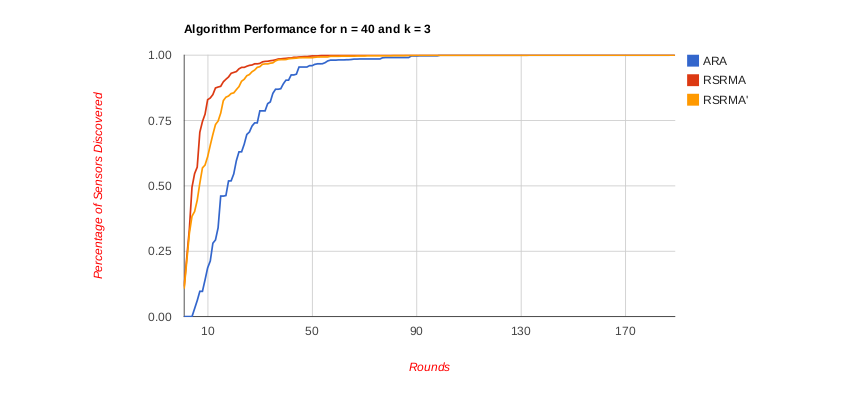
\includegraphics[height = 8cm]{pics/graph40k3.png}\\[0.5cm]    
\label{fig:n40k3}
\end{figure}

\begin{figure}[ht]
\caption{}
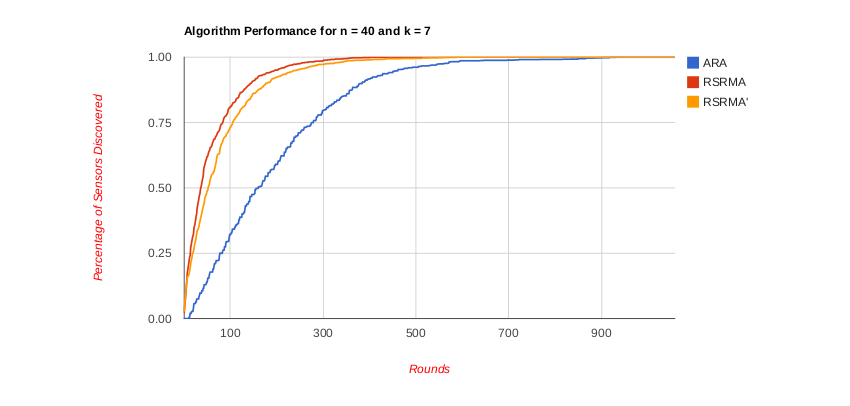
\includegraphics[height = 8cm]{pics/graph40k7.png}\\[0.5cm]   
\label{fig:n40k7} 
\end{figure}

\begin{figure}[ht]
\caption{}
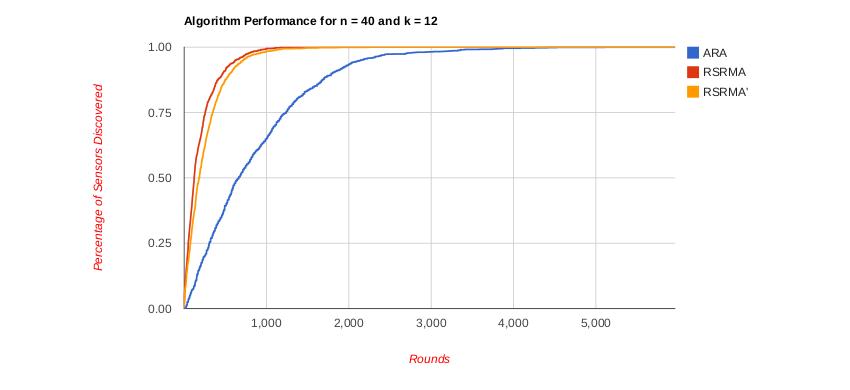
\includegraphics[height = 8cm]{pics/graph40k12.png}\\[0.5cm] 
\label{fig:n40k12}   
\end{figure}

At extremely low numbers of sensors, such as 10 (\ref{fig:n10k3}, \ref{fig:n10k7}, and \ref{fig:n10k12}) RSRMA and RSRMA' are difficult to distinguish. RSRMA starts out a bit quicker but by the end they are neck and neck. ARA is again the poor performer, but gets a boost at low k values.

\begin{figure}[ht]
\caption{}
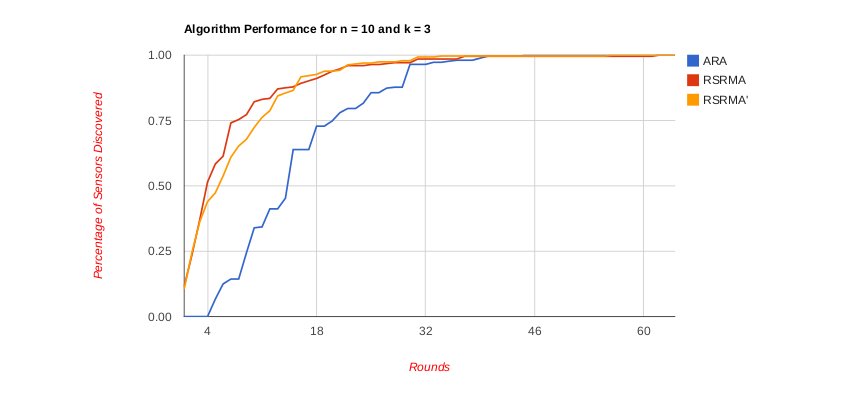
\includegraphics[height = 8cm]{pics/graph10k3.png}\\[0.5cm]    
\label{fig:n10k3}
\end{figure}

\begin{figure}[ht]
\caption{}
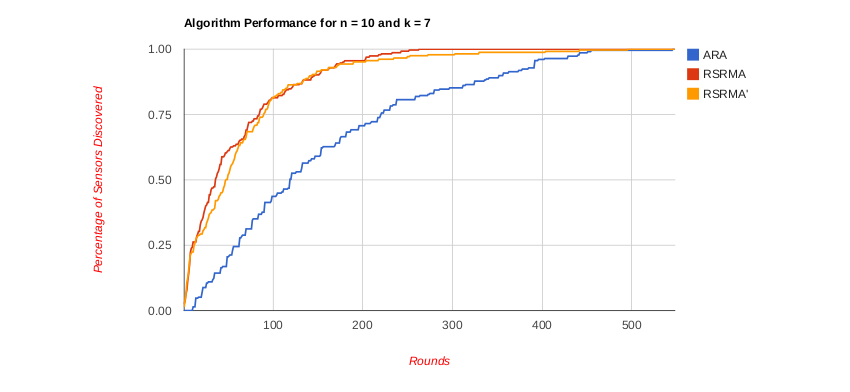
\includegraphics[height = 8cm]{pics/graph10k7.png}\\[0.5cm]   
\label{fig:n10k7} 
\end{figure}

\begin{figure}[ht]
\caption{}
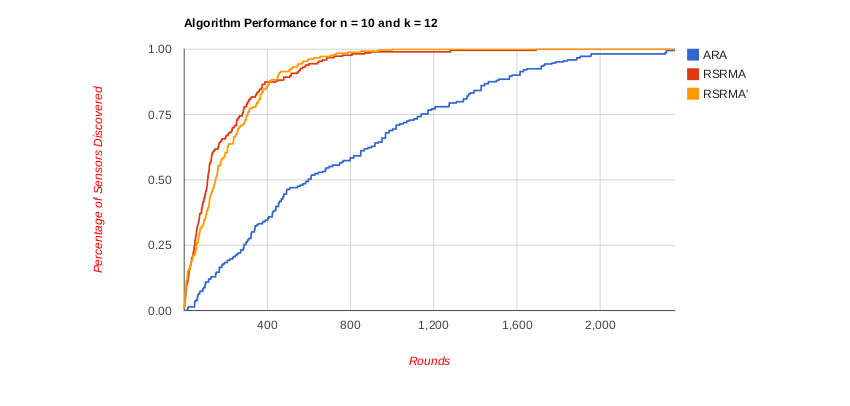
\includegraphics[height = 8cm]{pics/graph10k12.png}\\[0.5cm] 
\label{fig:n10k12}   
\end{figure}


